
\section{DIFRACCIÓN}
\subsection{Concepto}

\begin{frame}{DIFRACCIÓN}
    \framesubtitle{Concepto}
    Un objeto opaco que se interpone entre una fuente de luz y una superficie, una pared por ejemplo, la sombre que se observa no es totalmente nítida\footnote{\bibentry{sears}}.
    \begin{figure}[H]
		\centering
		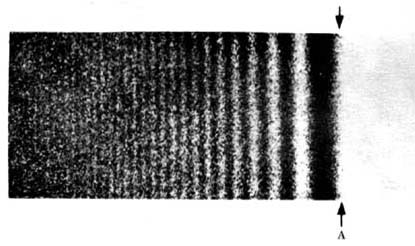
\includegraphics[scale=1]{david/Shadow.jpg}
		\caption{Acercamiento al borde de una sombra \footnotemark{}.}
	\end{figure}
    \footnotetext{\bibentry{Shadow}}
    \begin{itemize}
        \item Fallan las predicciones de la óptica geométrica.
        \item Franjas brillantes y oscuras alternadas.
    \end{itemize}
    \vspace{-5mm}
\end{frame}

\begin{frame}{DIFRACCIÓN}
    \framesubtitle{Concepto}
    También se puede definir como los patrones de interferencia que se forman cuando la luz incide en una barrera que cuenta con una abertura o un borde. Pero, en general, aplica para todo tipo de ondas \footnote{\bibentry{sears}}.
    \begin{figure}[H]
		\centering
		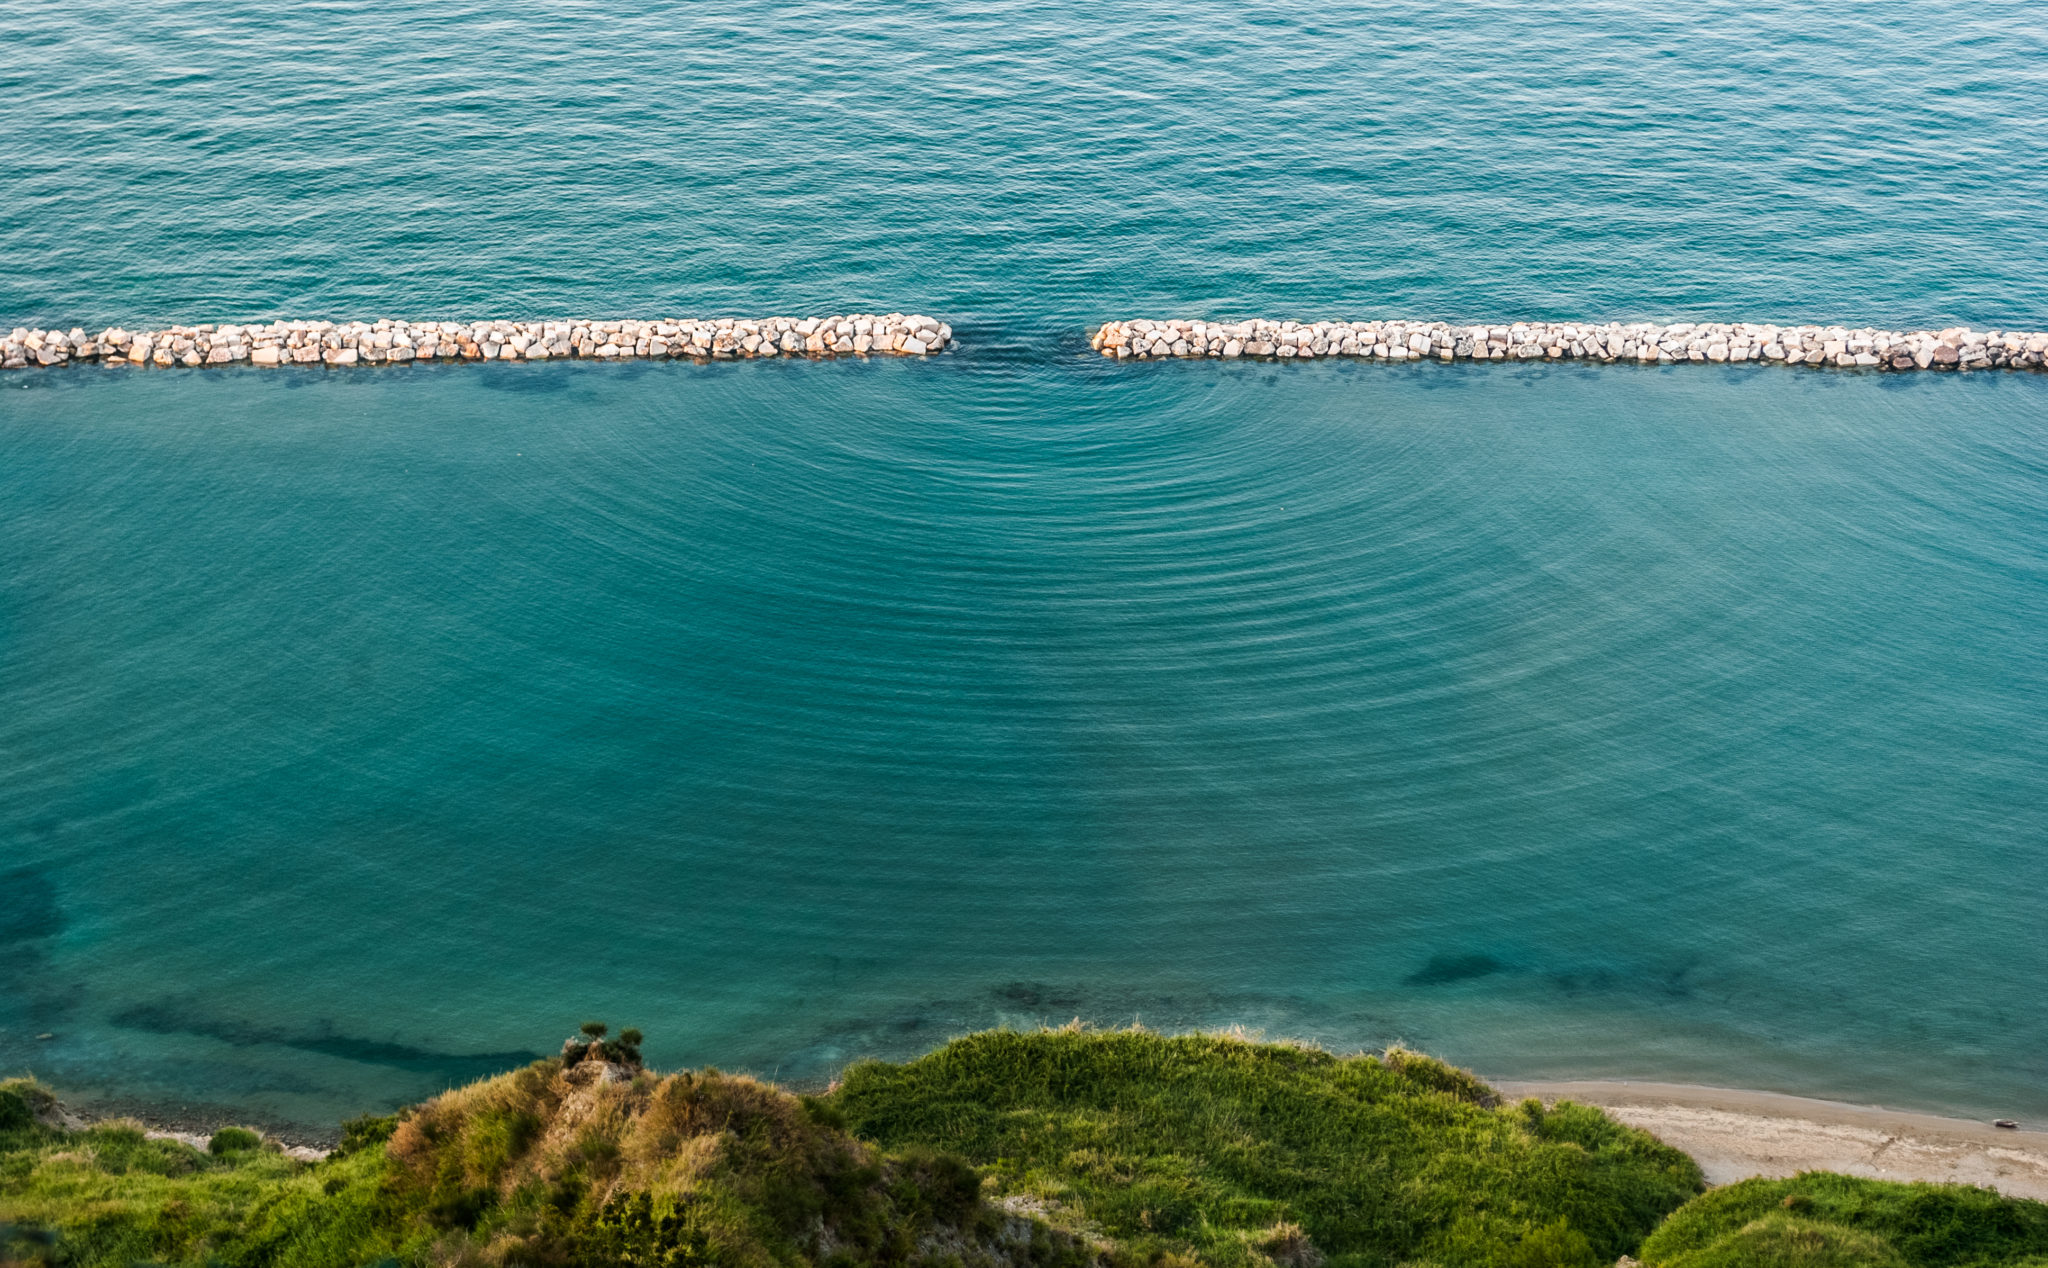
\includegraphics[scale=0.35]{david/waterwave.jpg}
		\caption{Difracción de una onda en el mar\footnotemark{}.}
	\end{figure}
    \vspace{-1cm}\footnotetext{\bibentry{waterwave}}
\end{frame}

\begin{frame}{DIFRACCIÓN}
    \framesubtitle{Principio de Fresnel-Huygens}
    \textit{"Todo punto de un frente de onda inicial puede considerarse como una fuente de ondas esféricas secundarias que se extienden en todas las direcciones con la misma velocidad, frecuencia y longitud de onda que el frente de onda del que proceden" \footnote{\bibentry{hecht}}}.
    \begin{figure}
        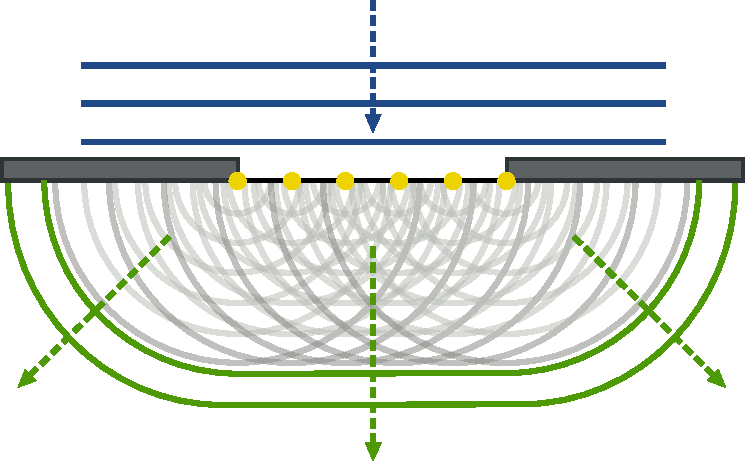
\includegraphics[scale=0.53]{david/huygens.pdf}
        \caption{Principio de Huygens a través de una rendija.}
    \end{figure}
\end{frame}

\subsection{Patrón de Difracción}
\begin{frame}{DIFRACCIÓN}
    \framesubtitle{Patrón de Difracción}
    Imagen de la modulación de la intensidad de la onda debido a la difracción.  El patrón de difracción se construye a partir de la superposicion de todas las ondas que plantea Fresnel-Huygens\footnote{\bibentry{hecht}}.
    \begin{figure}
        \centering
        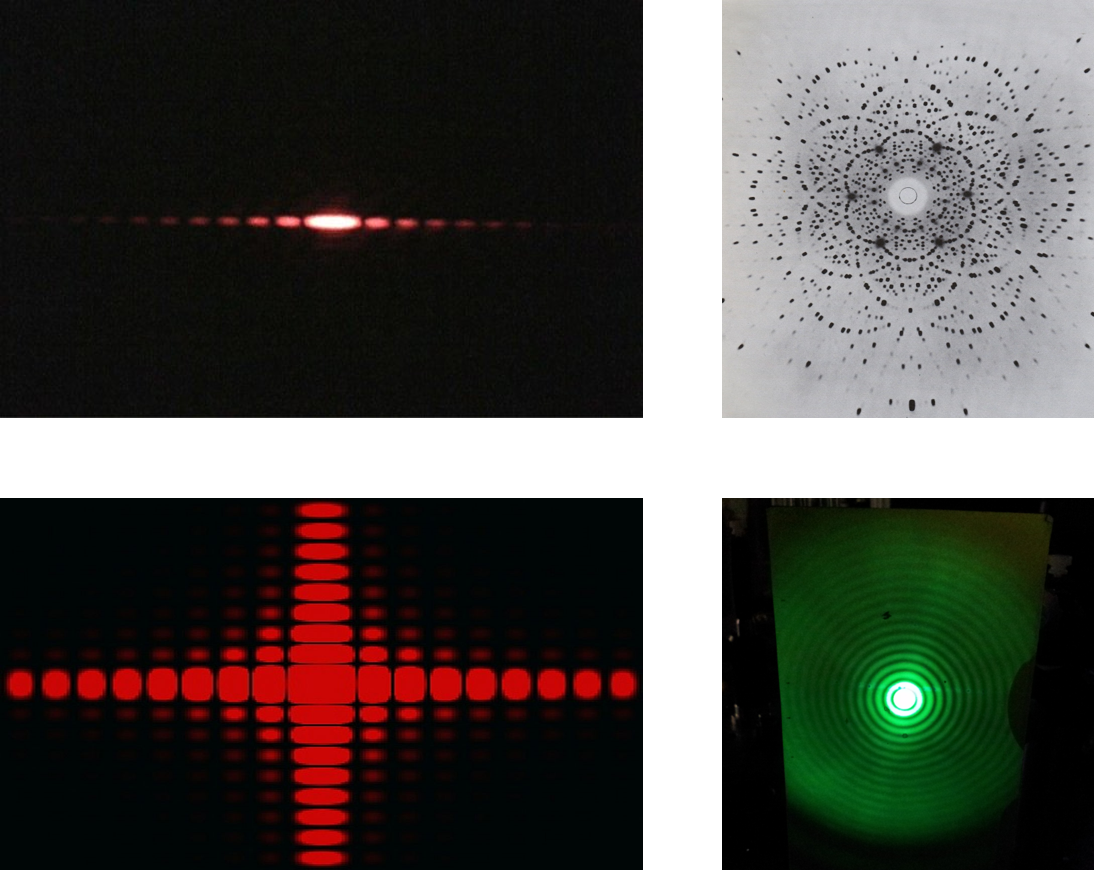
\includegraphics[scale=0.295]{david/Diff.png}
        \caption{Diferentes patrones de difracción.}
    \end{figure}
    \vspace{-2cm}
\end{frame}

\subsection{Enfoques}
\begin{frame}{DIFRACCIÓN}
    \framesubtitle{Enfoques}
    \begin{multicols}{2}
        \textbf{Fresnel}\\
            Se considera la curvatura de las ondas salientes de la abertura de difracción. Normalmente ocurre cuando la abertura está muy cerca a la pantalla de observación.
        \vfill\null
        \textbf{Fraunhofer}\\
            Se considera difracción de Fraunhofer cuando las ondas salientes de la rendija con casi planas comparadas con la fuente\footnote{\bibentry{hecht}}.
    \end{multicols}
    \begin{figure}[H]
        \centering
        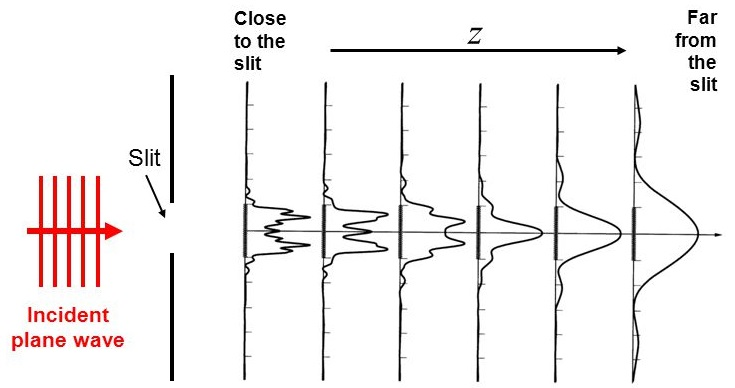
\includegraphics[scale=0.3]{david/enfoques.jpg}
        \caption{Intensidad de acuerdo al enfoque de estudio\footnotemark{}.}
    \end{figure}
    \footnotetext{\bibentry{Wilcox}}
    \vspace{-1.5cm}
\end{frame}

\begin{frame}{DIFRACCIÓN}
    \framesubtitle{¿Qué tanto se difracta una onda?}
    La difracción depende de qué tan comparable sea un obstáculo con la longitud de onda.
    \begin{figure}
        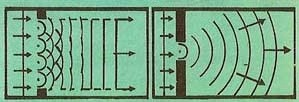
\includegraphics[scale=0.5]{david/wavelength.jpg}
        \caption{Comparación de una onda incidente respecto a rendijas.}
    \end{figure}

    \begin{figure}
        \centering
        \begin{subfigure}[H]{0.25\textwidth}
            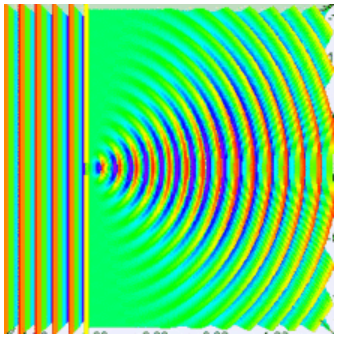
\includegraphics[width=\linewidth]{david/narrow.PNG}
        \end{subfigure}
        \hspace{2mm}
        \begin{subfigure}[H]{0.25\textwidth}
            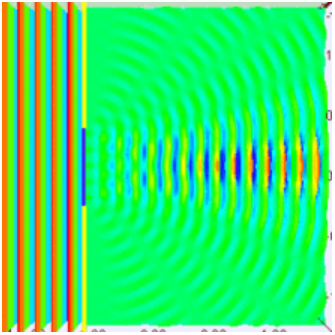
\includegraphics[width=\linewidth]{david/wide.PNG}
        \end{subfigure}
        \caption{Propagación de acuerdo a las rendijas\footnotemark{}.}
    \end{figure}
    \vspace{-1cm}\footnotetext{\bibentry{wikiwave}}

\end{frame}

\subsection{Experimento de una Rendija}
\begin{frame}{DIFRACCIÓN}
    \framesubtitle{Experimento de una Rendija}
    Hay una onda incidente en la abertura, la abertura se considera como una fuente continua de ondas esféricas\footnote{\bibentry{sears}}.
    \begin{equation}
        I=I_0\left\{\frac{\sin\left[\pi a \left(\sin\theta\right)/\lambda\right]}{\pi a\left(\sin\theta\right)/\lambda}\right\}^2
    \end{equation}
    \vspace{-5mm}
    \begin{figure}
        \centering
        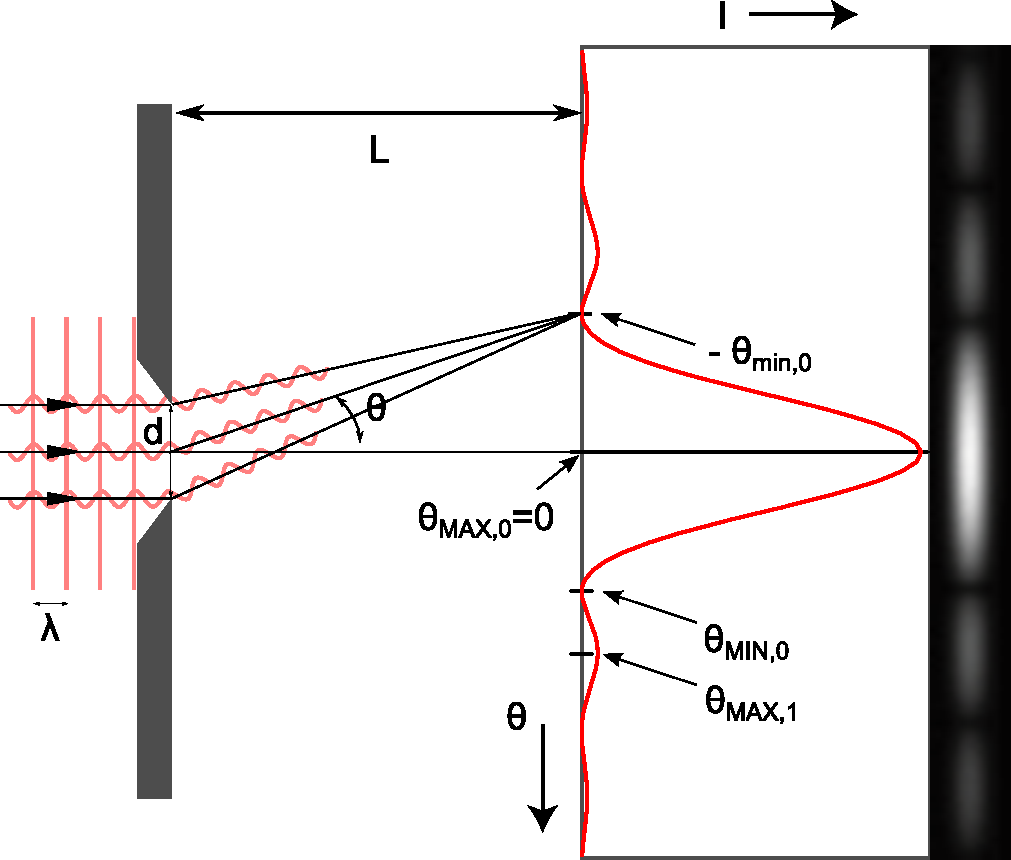
\includegraphics[scale=0.25]{david/singleSlit.pdf}
        \caption{Difracción, intensidad y patrón de difracción para una rendija.}
    \end{figure}
    \vspace{-2cm}
\end{frame}

\subsection{Experimento de Young}

\begin{frame}{DIFRACCIÓN}
    \framesubtitle{Experimento de Young}
    \textbf{¿Qué esperaríamos ver?\\}
	Si la luz se comportara como una partícula, se esperaría observar:
	 \begin{figure}
         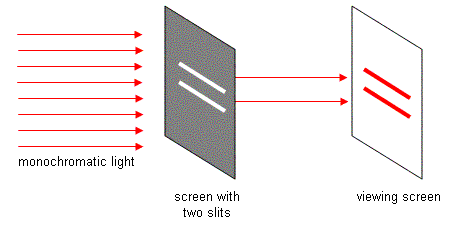
\includegraphics[scale=0.7]{juanse/young_particle.png}
         \caption{Resultado esperado del modelo como partícula\footnotemark{}.}
     \end{figure}
     \footnotetext{\bibentry{young1}}
\end{frame}

\begin{frame}{DIFRACCIÓN}
    \framesubtitle{Experimento de Young}
    \begin{figure}
        \centering
        \begin{subfigure}[H]{0.4\textwidth}
            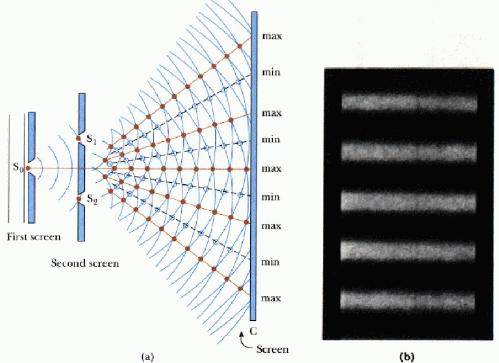
\includegraphics[width=\linewidth]{juanse/waves.png}
            \caption{Patrón de Interferencia\footnotemark{}.}
        \end{subfigure}
        \hspace{2cm}
        \begin{subfigure}[H]{0.4\textwidth}
            \only<1>{}
            \only<2>{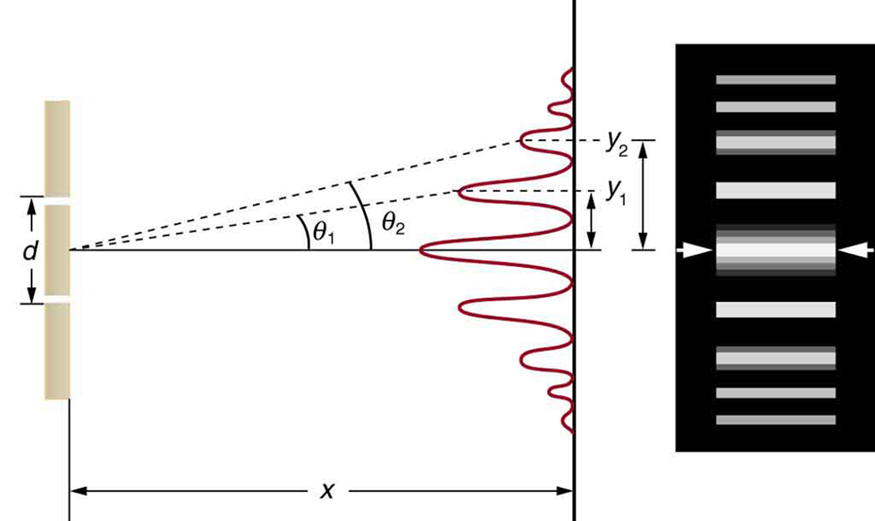
\includegraphics[width=\linewidth]{juanse/waves2.jpg}
            \caption{Patrón de Intensidad\footnotemark{}.}}
        \end{subfigure}
    \end{figure}
    \addtocounter{footnote}{-1}
    \footnotetext{\bibentry{youngwaves}}
    \addtocounter{footnote}{1}
    \footnotetext{\bibentry{youngwaves2}}
\end{frame}


\subsection{Difracción de Rayos X}
\begin{frame}{DIFRACCIÓN}
    \framesubtitle{Rayos X}
    Los rayos X fueron descubiertos por Wilhelm Röntgen en 1895; tienen longitudes del orden de $10^{-10}\,m$. Pueden utilizarse para determinar defectos en componentes técnicos, como tuberías, turbinas, motores, paredes, vigas, y en general casi cualquier elemento estructural\footnote{\bibentry{sears}}.
    \begin{figure}
        \centering
        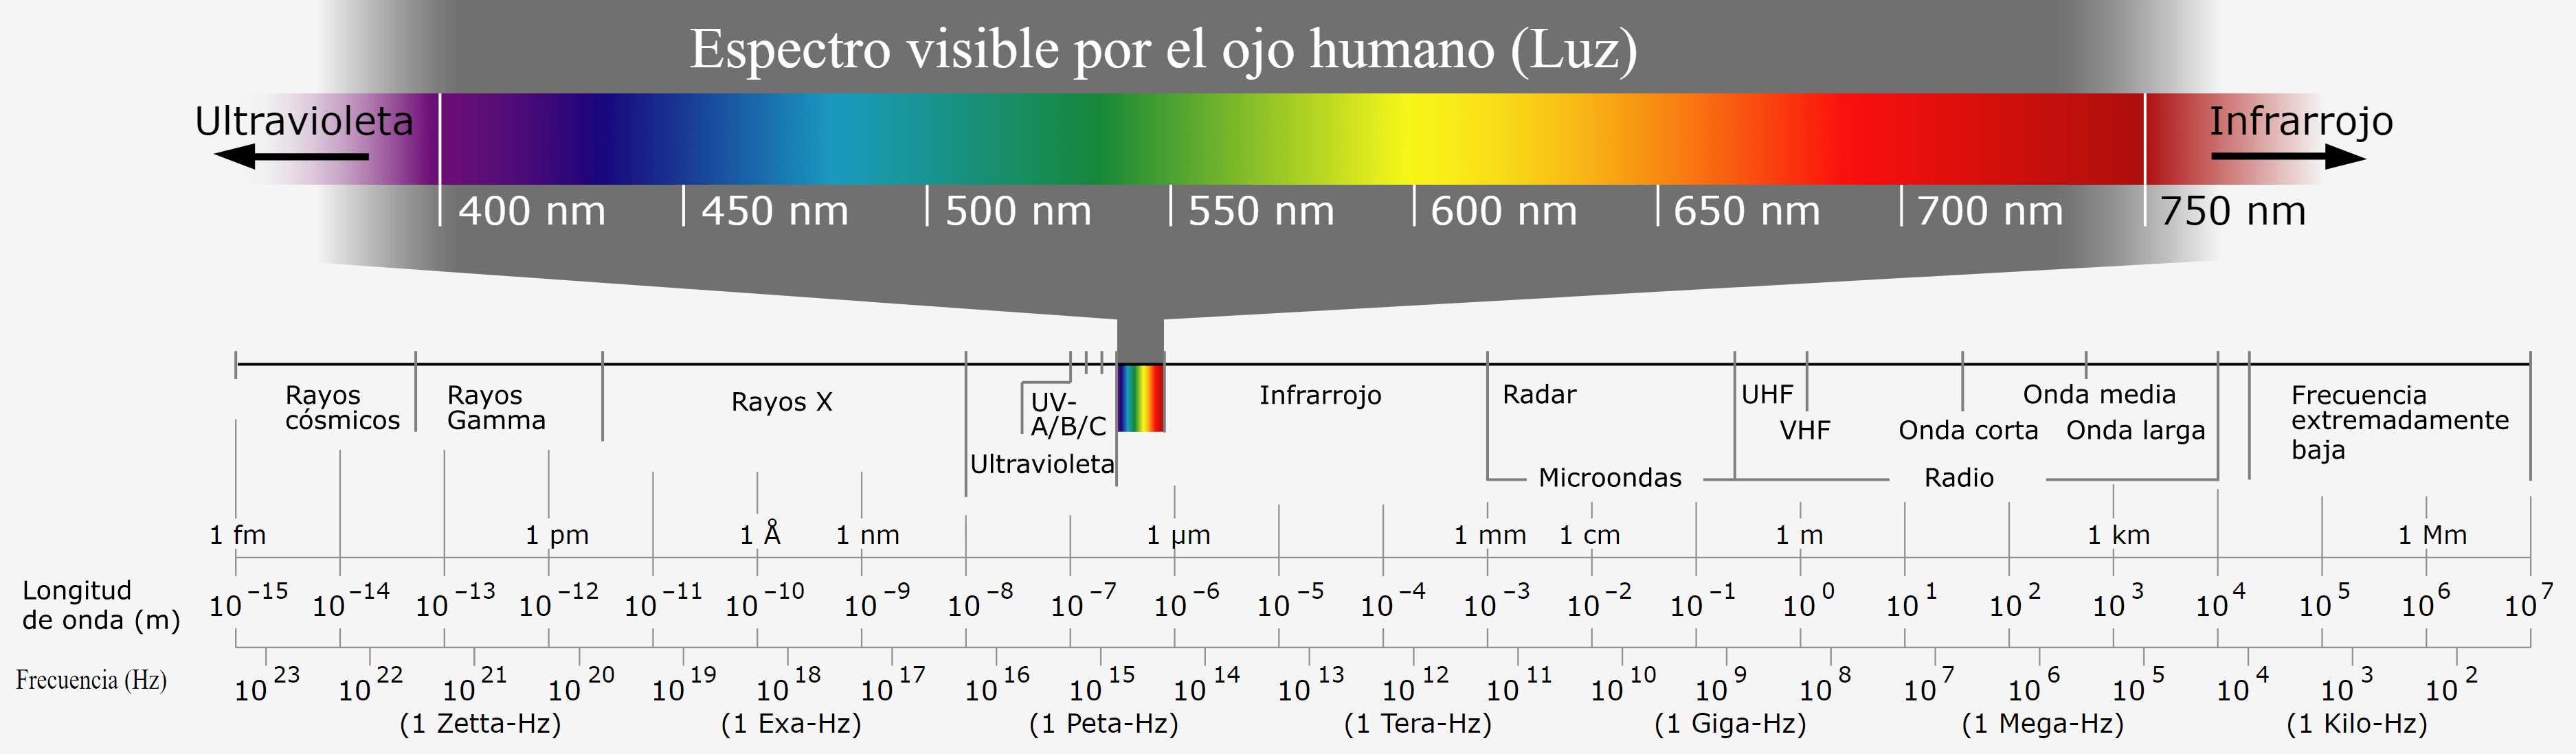
\includegraphics[scale=0.084]{david/espectro.png}
        \caption{Espectro electromagnético\footnotemark{}.}
    \end{figure}
    \vspace{-5mm}\footnotetext{\bibentry{espectro}}
\end{frame}



\begin{frame}{DIFRACCIÓN}
    \framesubtitle{Difracción de Rayos X}
    En 1912, Max von Laue propuso la idea de que un cristal podría servir como una rejilla de difraccion tridimensional para los rayos X.
    \begin{figure}[H]
		\centering
		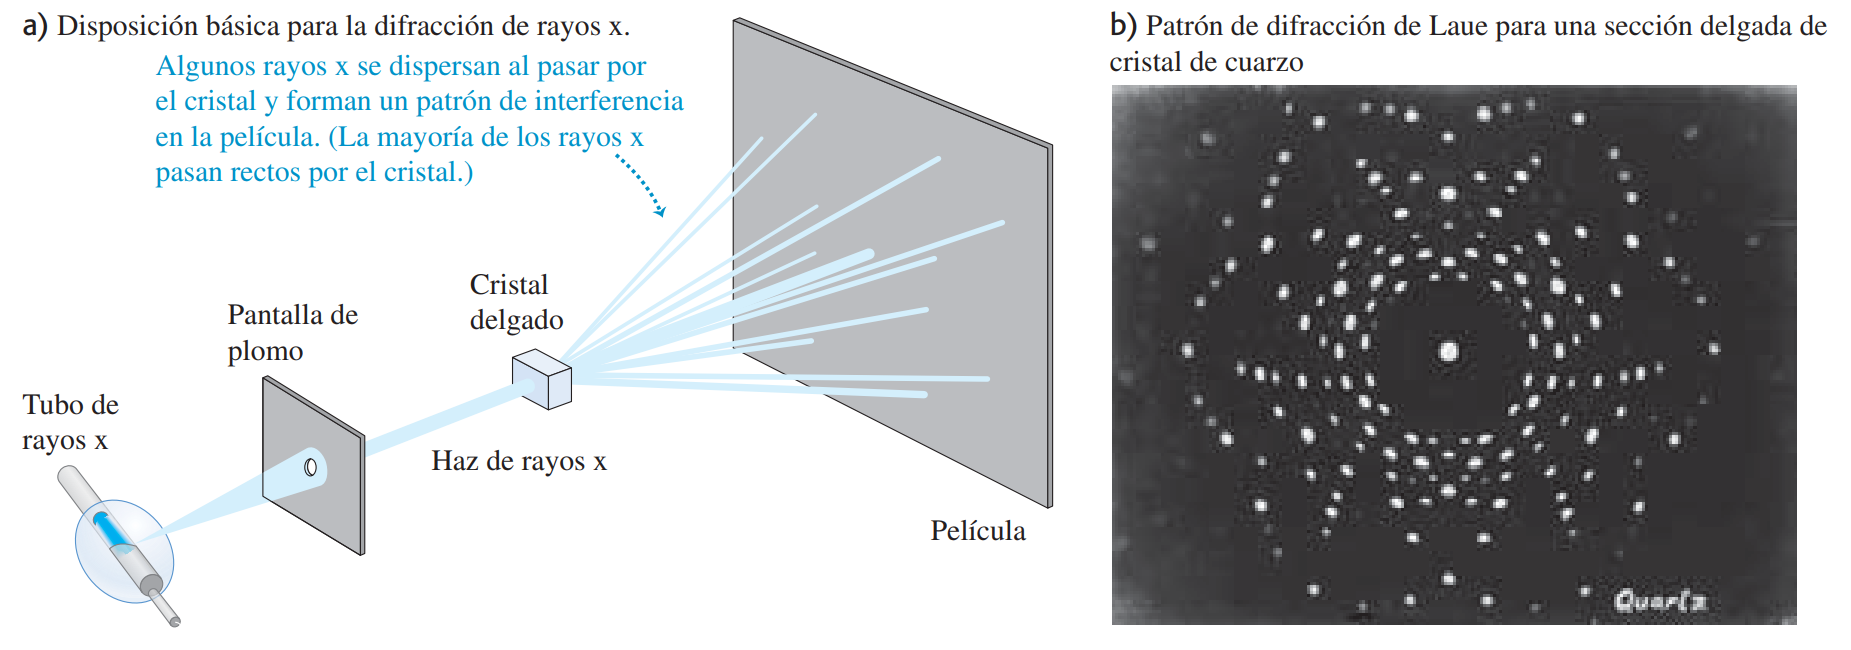
\includegraphics[scale=0.1975]{david/Laue.PNG}
		\caption{Experimento de Laue \footnotemark{}.}
	\end{figure}
    \footnotetext{\bibentry{sears}}
    Resultó en la prueba experimental de que los rayos X son, en efecto, una onda electromagnética.
    \vspace{-1cm}
\end{frame}

\begin{frame}{DIFRACCIÓN}
    \framesubtitle{Difracción de Rayos X}

\end{frame}
